\section{Performance and Accuracy Evaluation}
\label{sec:performance-evaluation}

Tests have been conducted following the performance and accuracy testing methodology defined in Section \ref{subsec:performance-and-accuracy-testing}.
These tests leveraged the \ac{grs} identity registration and classification \ac{api} endpoints to automate the training and testing of its classification model using a secondary dataset.
All tests were conducted on the benchmark machine (laptop) defined in Table \ref{tab:benchmark-system-specs}, targeting test \#PT2 in Table \ref{tab:performance-tests}.

The CASIA-B dataset is a well-known dataset, created between 2012 and 2014, used for benchmarking in \ac{gr} research.
It contains 124 subjects captured multiple times from eleven (11) different angles (0$\deg$, 18$\deg$, ..., 180$\deg$).
Subjects were captured in three different conditions: normal, wearing a coat, and carrying a bag \parencite{fuCASIABPoseCASIABPose2023}.

For these tests, only the normal walking condition, and 90$\deg$ angle (perpendicular lateral view) samples were used, resulting in six samples per subject.
These samples were split into training and testing sets, with three samples used for training and three used for testing, with no overlap between the two sets.
The final dataset metrics are listed below.
Although diversity details are not specified, subjects are known to be of varying age and sex.

\begin{itemize}
    \item \textbf{Subjects}: 124 unique individuals
    \item \textbf{Samples per Subject}: 6 gait sequences
    \item \textbf{Total Samples}: 744
    \item \textbf{Split}: 50\% Training (3 samples/subject), 50\% Testing (3 samples/subject)
\end{itemize}

For anonymity, the publically available dataset is preprocessed into binary silhouette sequences (as implemented in this system in Section \ref{subsec:background-subtraction-and-person-detection}).
To prepare the dataset for training and testing, the silhouette normalisation and \ac{gei} creation process was extracted from the \ac{grs}' \codeword{GaitProcessor} class, and applied to the dataset in a custom Python script.
This produced a dataset of 744 \ac{gei} images, split into training and testing sets of 372 images each, labelled with the subject's ID number.

Following dataset preparation, a script was created to automate the submission of each training sample to the \ac{grs}' \codeword{/api/register} endpoint, with the label defined as the subject's ID number --- see Appendix \ref{app:gait-recognition-server-training-function}
Training was successful for all 372 samples, with no failed submissions.
The process completed in 16 minutes and 57 seconds, with an average registration time of 2.6 seconds.

The time taken to register each sample was recorded to enable evaluation of test \#PT4 in Table \ref{tab:performance-tests}.
Figure \ref{fig:registration-times} below shows the distribution of registration times for each sample, with a mean of 2.6 seconds and a median of 2.9 seconds.

\begin{figure}[H]
    \centering
    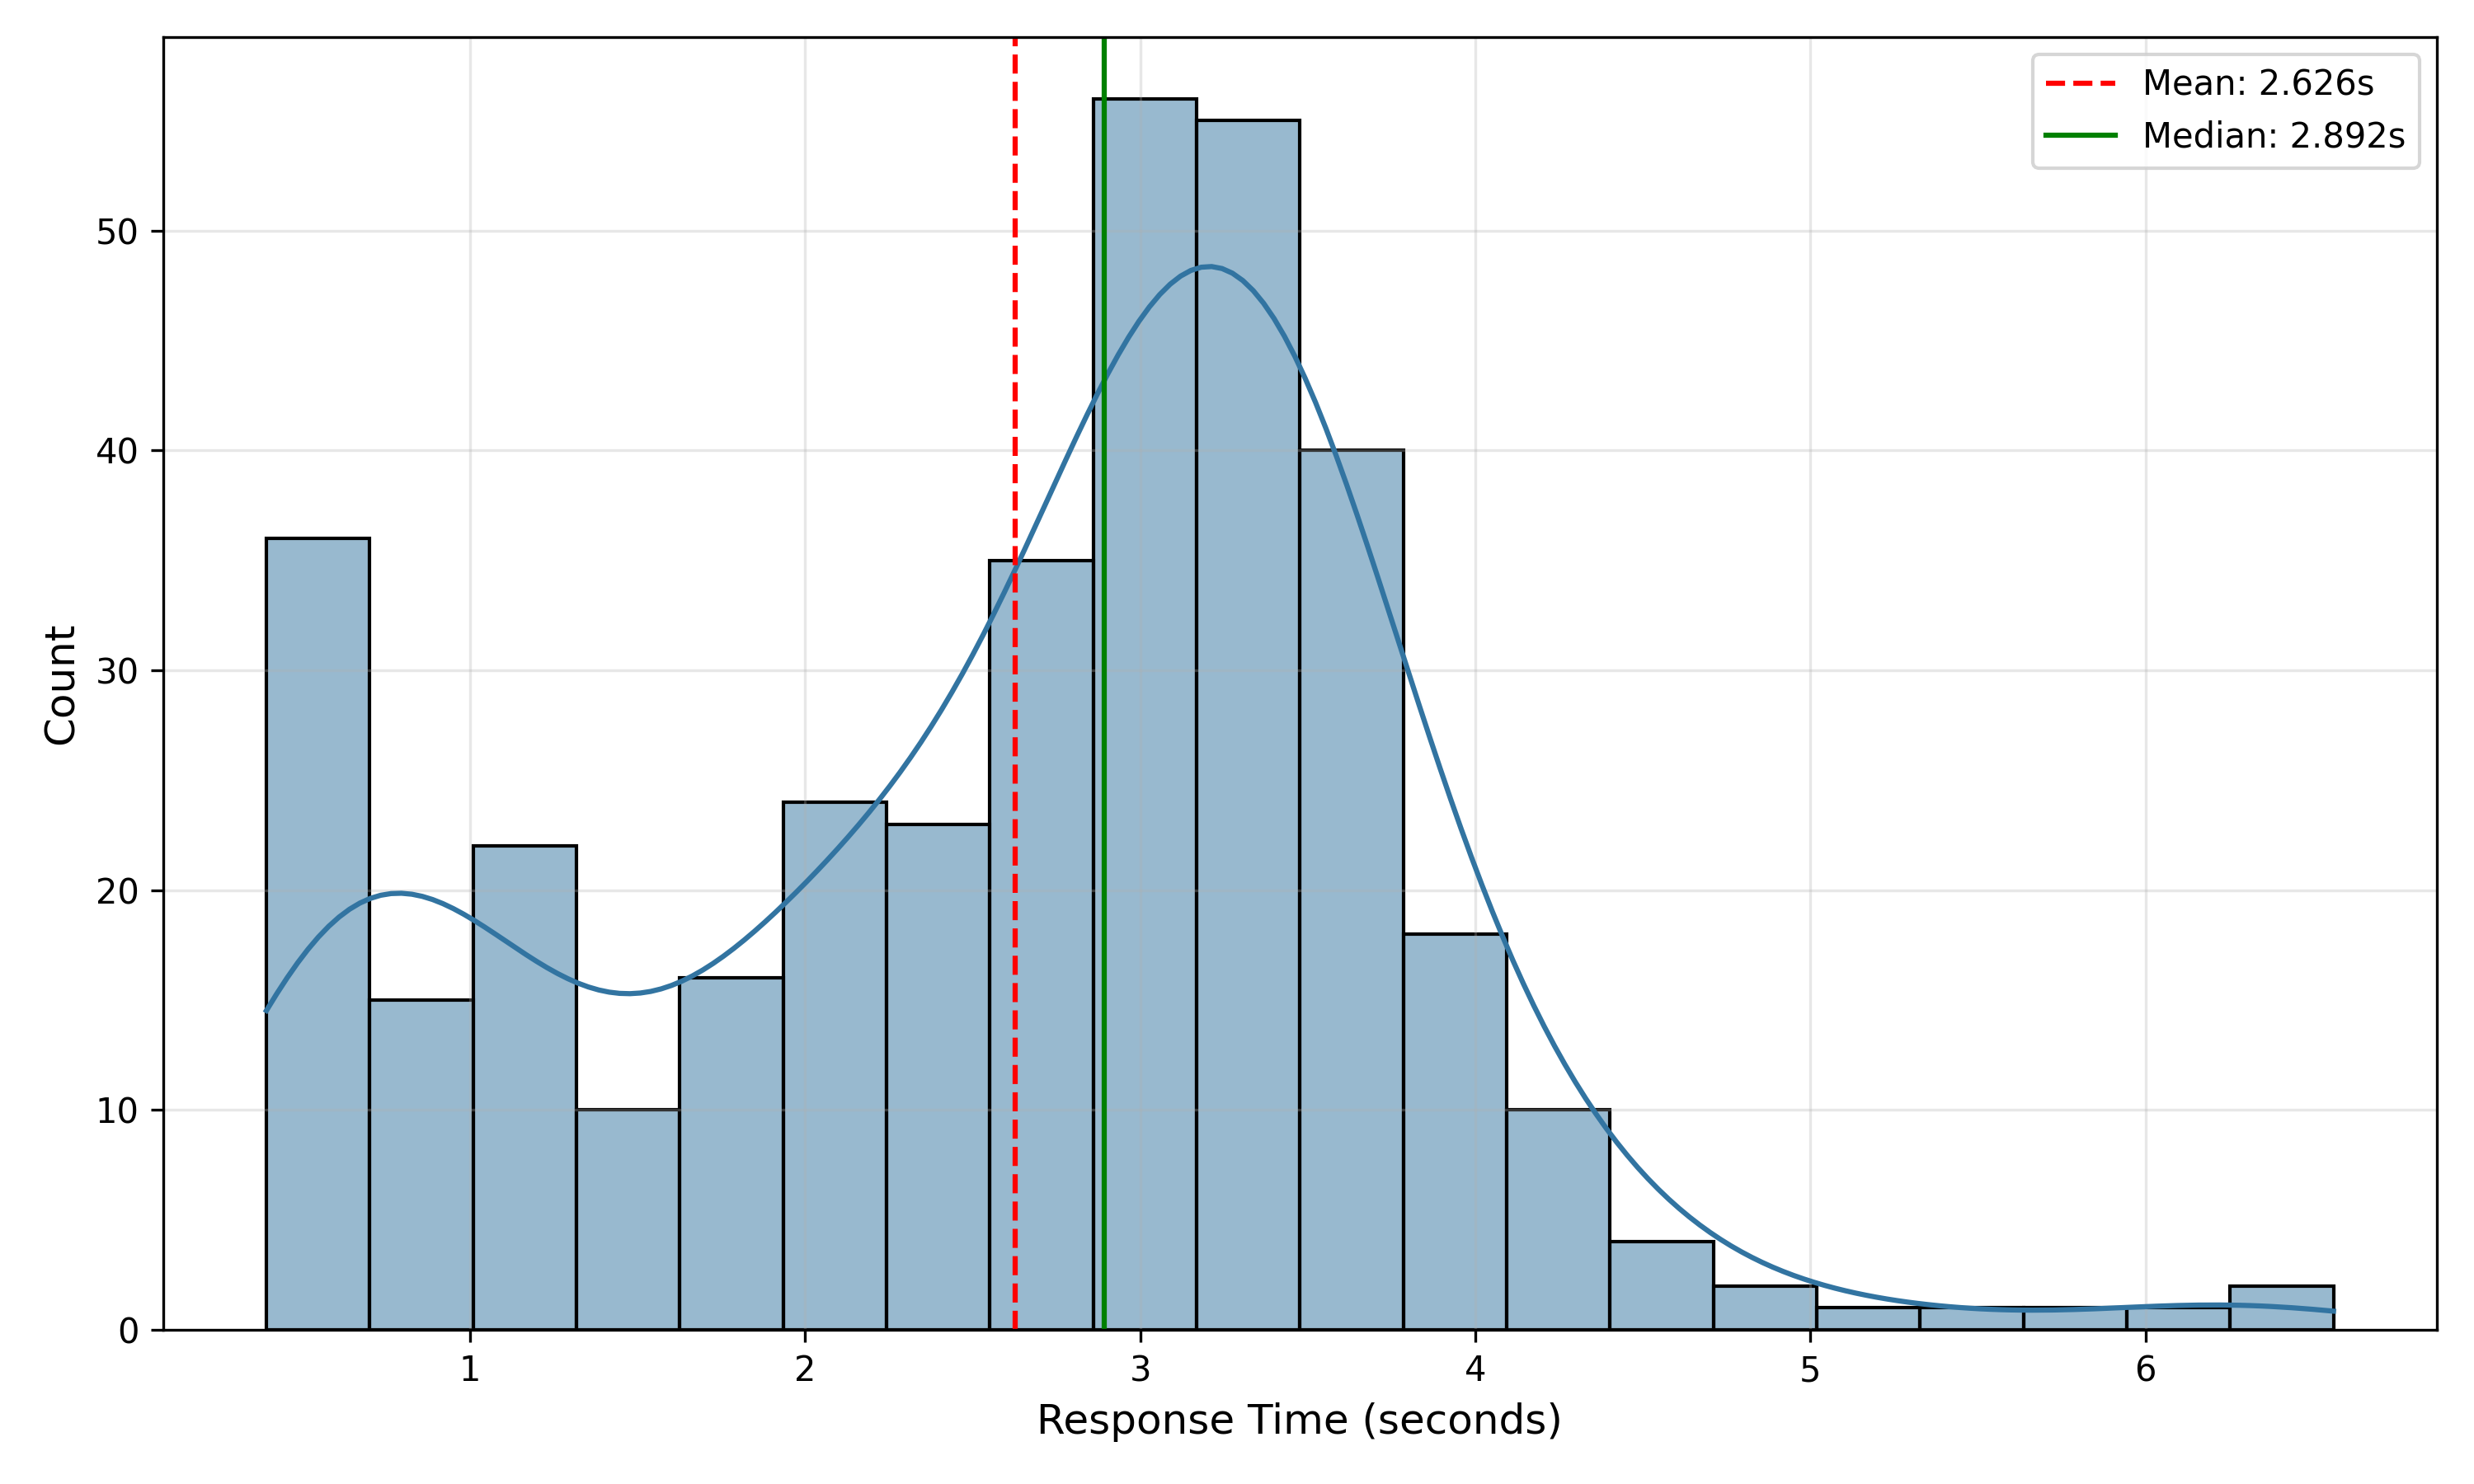
\includegraphics[width=0.8\textwidth]{assets/registration_analysis_response_time_distribution.png}
    \caption{GEI Registration Response Time Distribution}
    \label{fig:registration-times}
\end{figure}

It was observed that as the size of the \ac{grs}' classification model grew, registration time increased.
This is likely reflects the overhead introduced by retraining the model incrementally as new \ac{gei} samples are registered.

Figure \ref{fig:registration-times-trend} below shows the trend of registration time as the number of samples in the \ac{grs}' classification model increased.

\begin{figure}[H]
    \centering
    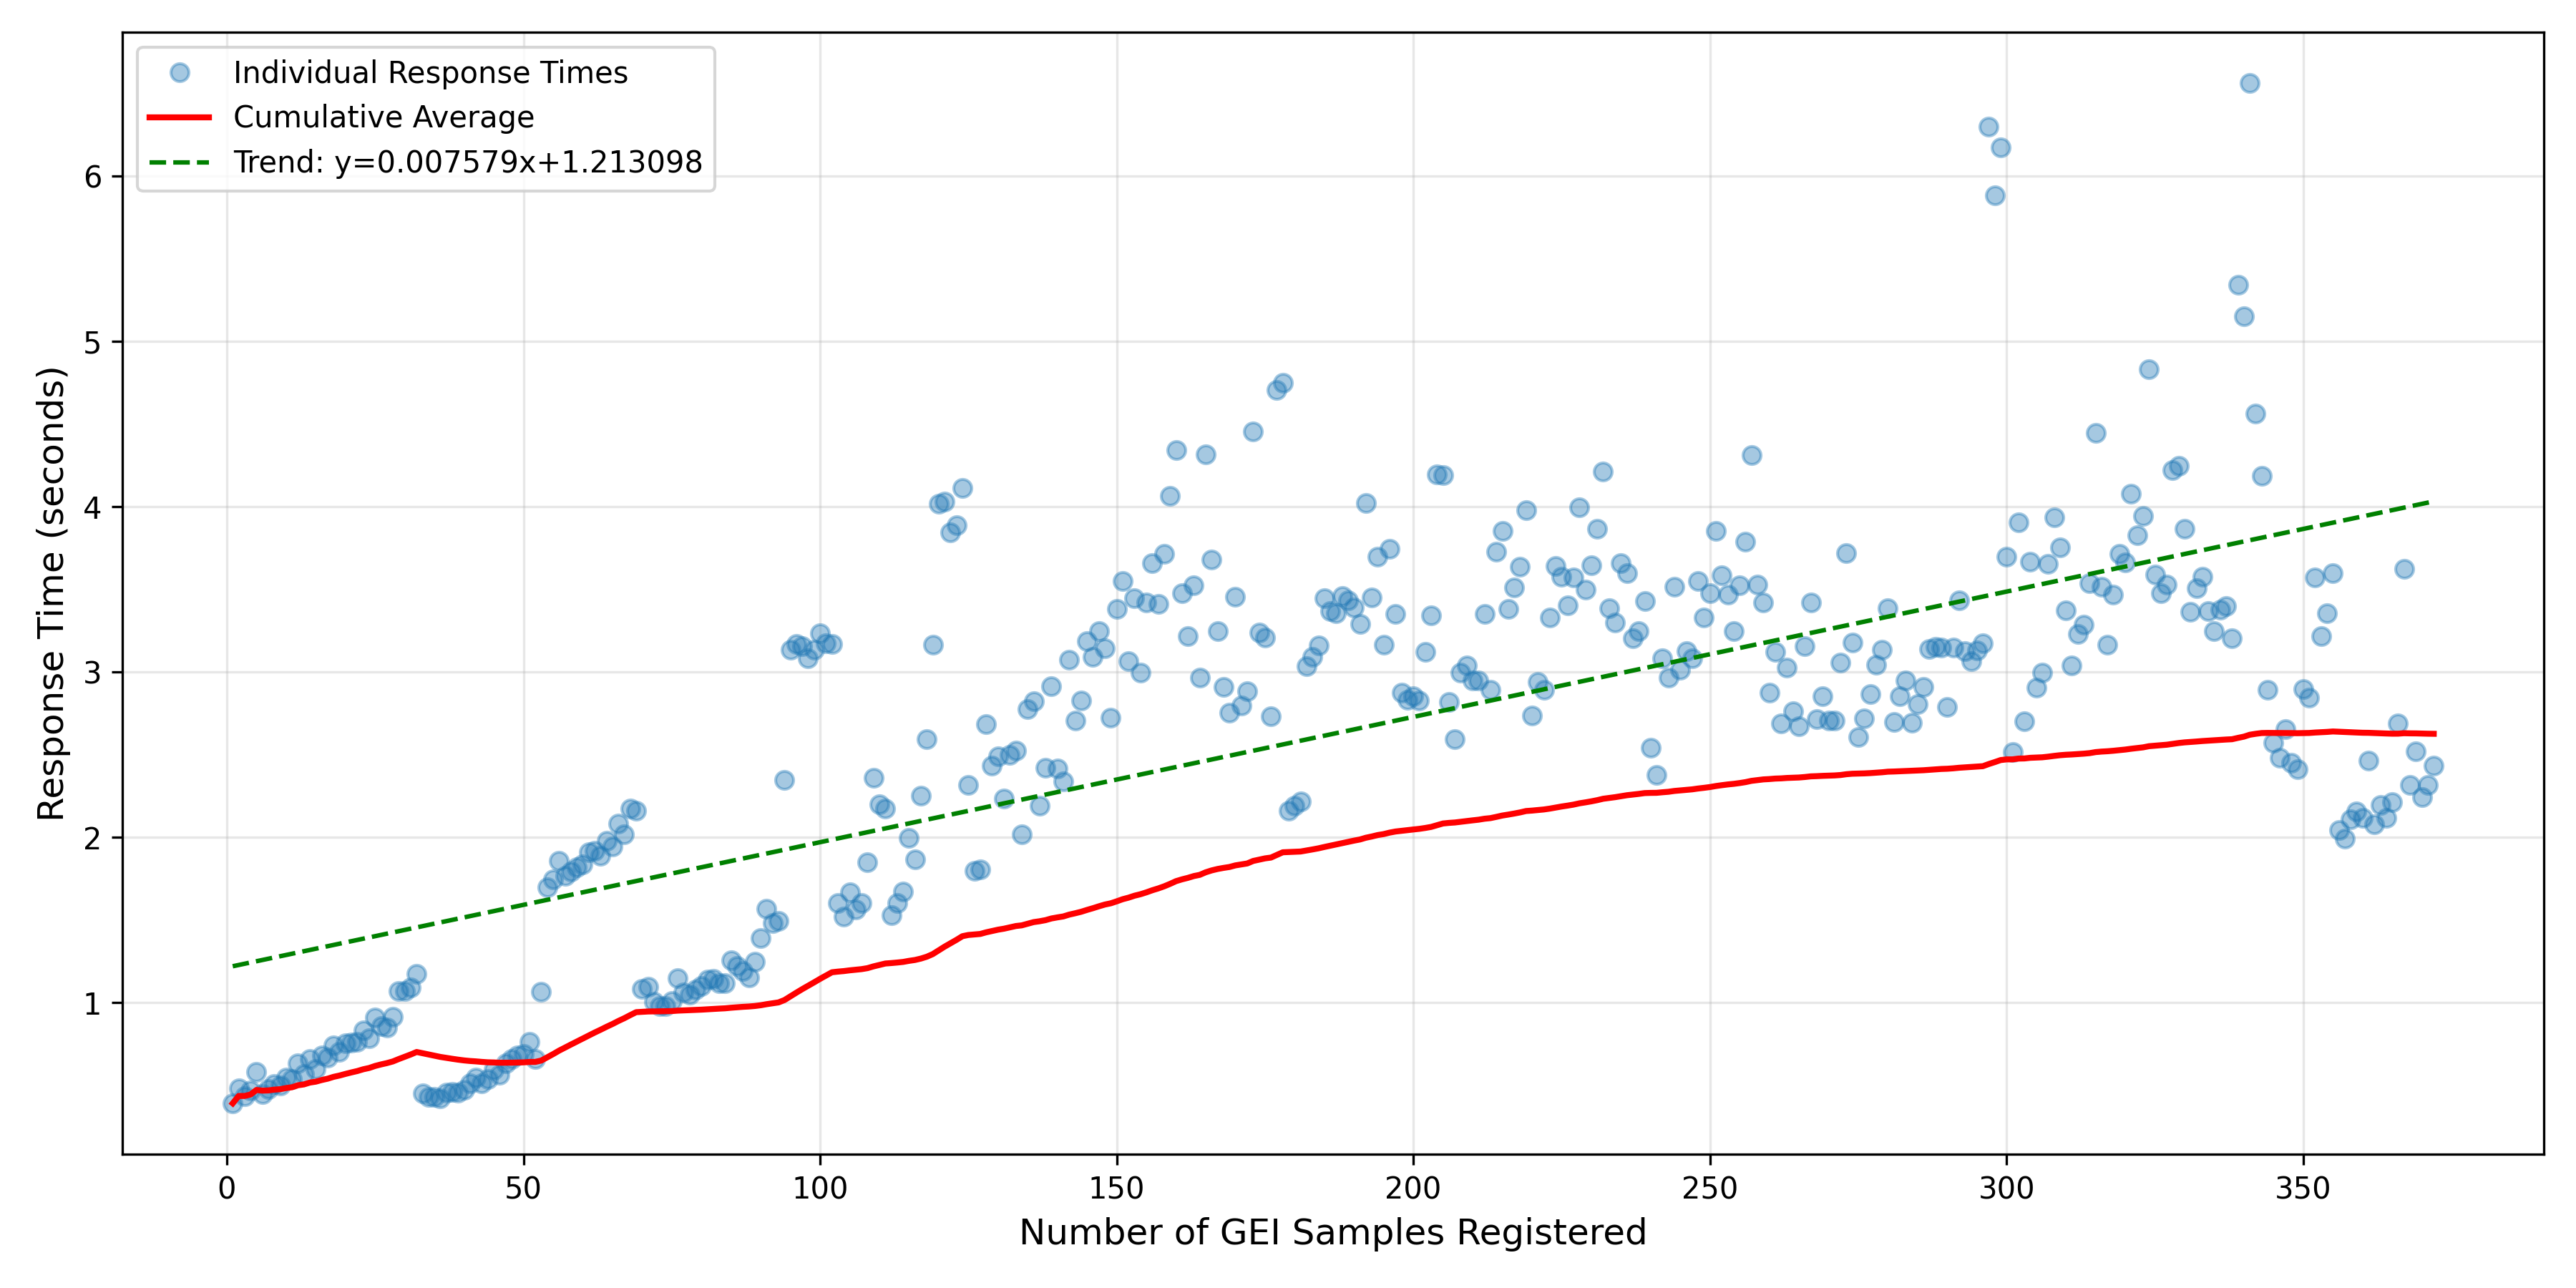
\includegraphics[width=0.8\textwidth]{assets/registration_analysis_response_time_trend.png}
    \caption{GEI Registration Response Time Trend}
    \label{fig:registration-times-trend}
\end{figure}

After training of the \ac{grs}' classification model was complete, another script was created to automate the submission of each testing sample to the \ac{grs}' \codeword{/api/classify} endpoint --- see Appendix \ref{app:gait-recognition-server-testing-function}
The classification results were then evaluated by comparing the predicted subject ID with the true subject ID for each sample.

By leveraging the prediction confidence score, an additional 'confidence threshold' metric was introduced to refine the analysis.
This allowed overall accuracy, and accuracy above an acceptable (75\%) confidence threshold to be evaluated.

The final results of this accuracy evaluation are shown in Table \ref{tab:standard-metrics} below:

\begin{table}[H]
    \begin{scriptsize}
        \centering
        \caption{Classification Accuracy Metric}
        \label{tab:standard-metrics}
        \begin{tabular}{|L{0.3\textwidth}|L{0.625\textwidth}|}
            \hline
            \textbf{Metric}            & \textbf{Result}  \\
            \hline
            \textbf{Accuracy}          & 0.9624 (96.24\%) \\
            \hline
        \end{tabular}
    \end{scriptsize}
\end{table}

The metrics above show that the \ac{grs}' classification model is able to correctly classify 96.24\% of samples.
This however does not account for the model's prediction confidence, which is a critical factor in \ac{gr} identification for security-sensitive applications, where false positives are not acceptable.
To assess accuracy above an 'acceptable confidence', a 75\% confidence threshold (also implemented in the \ac{acc} system's access provision output) was applied to the results.

The overall 'accepted' accuracy of the \ac{grs}' classification model after applying this threshold was found to be 72.04\%.
Of the 372 samples tested, 270 were classified above the confindence threshold (72.57\% of the test set), with 268 samples correctly classified, and 2 misclassifications, resulting in an above-threshold precision of 99.26\%.

Figure \ref{fig:confidence-distribution} below shows the confidence distribution across correct and incorrect classifications with the 75\% confidence threshold marked.

\begin{figure}[H]
    \centering
    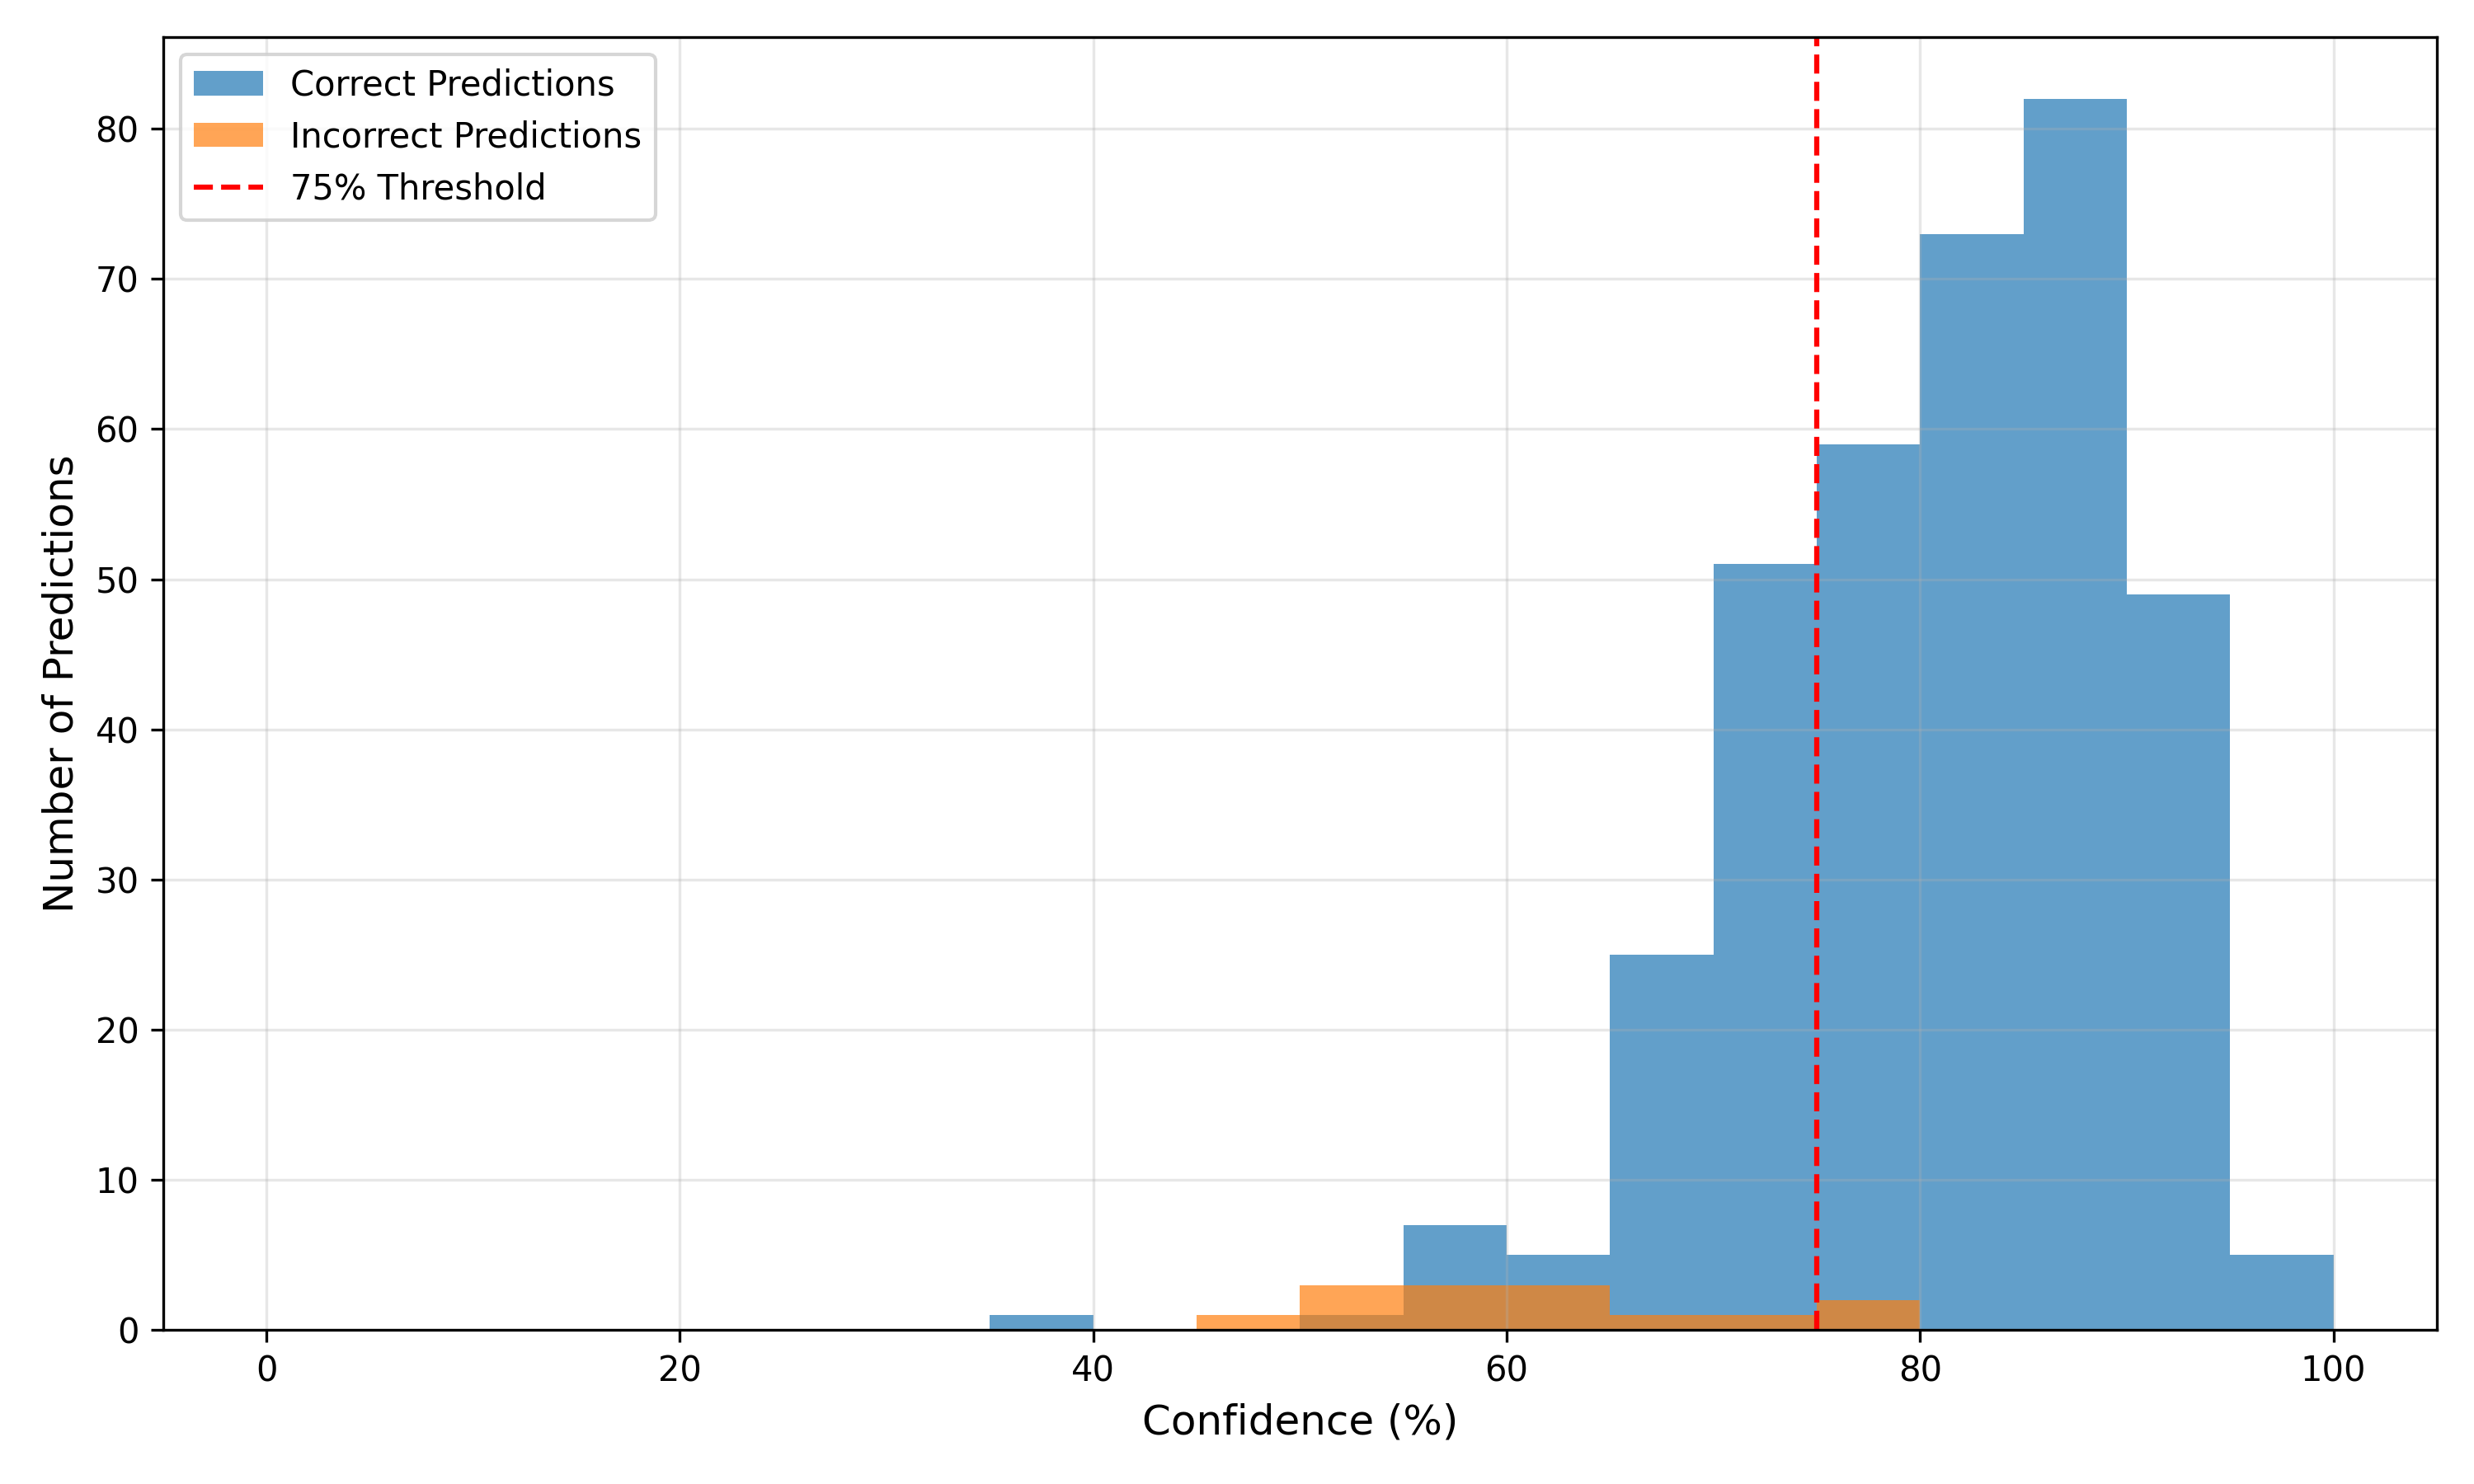
\includegraphics[width=0.8\textwidth]{assets/gei_analysis_confidence_distribution.png}
    \caption{GEI Classification Confidence Distribution}
    \label{fig:confidence-distribution}
\end{figure}

To enable evaluation of test \#PT3 in Table \ref{tab:performance-tests}, classification request response times were recorded.
Figure \ref{fig:classification-times} below shows the response times for each sample, with a mean of 11.5 seconds.

\begin{figure}[H]
    \centering
    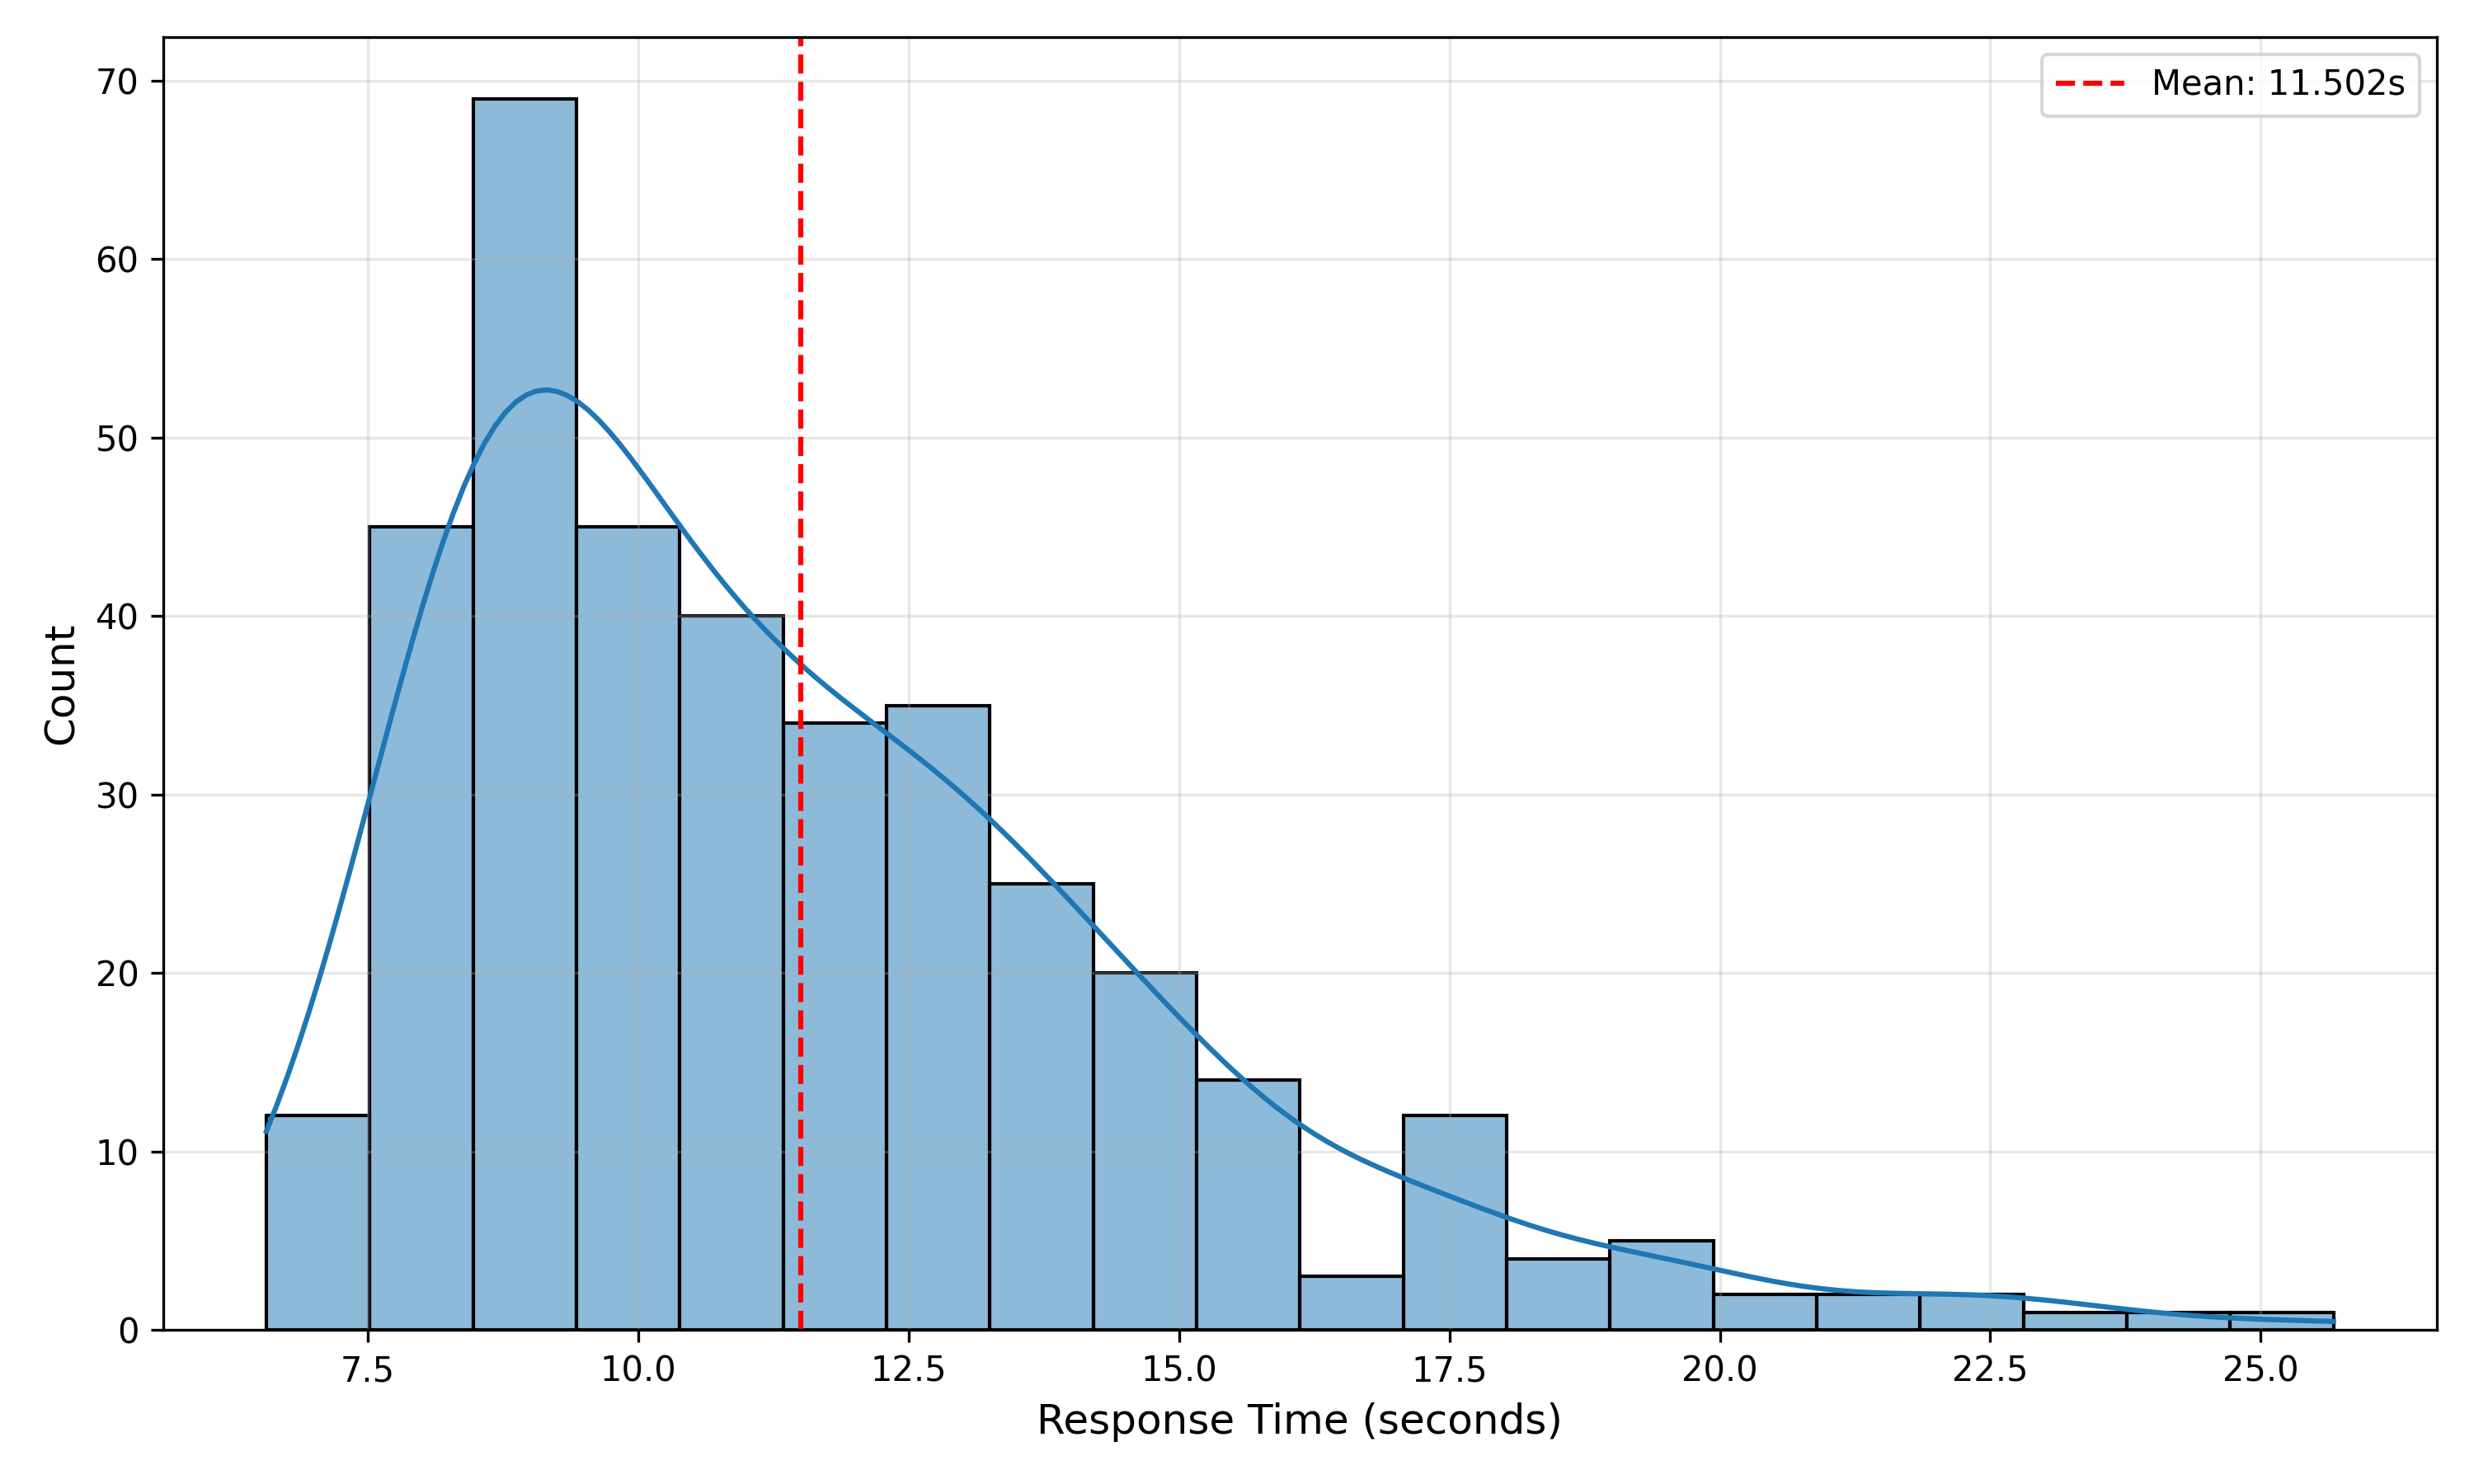
\includegraphics[width=0.8\textwidth]{assets/gei_analysis_response_time.png}
    \caption{GEI Classification Response Time Distribution}
    \label{fig:classification-times}
\end{figure}

Overall, these tests demonstrate that the system meets the performance and accuracy requirements set out in Section \ref{subsec:performance-and-accuracy-testing}:

\paragraph{PT1 --- Subject Diversity} Tests were conduted using the CASIA-B dataset, containing 124 unique subjects of varying age and sex.
\begin{tcolorbox}[colback=green!5, boxrule=0pt, frame empty]
    This demonstrates that the system is able to handle a diverse range of subjects, and is not biased towards any particular demographic.
\end{tcolorbox}

\paragraph{PT2 --- Hardware Requirements} Tests were conducted on the (consumer-grade) benchmark machine (laptop) defined in Table \ref{tab:benchmark-system-specs}.
\begin{tcolorbox}[colback=green!5, boxrule=0pt, frame empty]
    This demonstrates that the system is able to operate efficiently on hardware without significant processing power.
\end{tcolorbox}

\paragraph{PT3 --- Classification Speed} Tests were conducted to evaluate the speed of the system's classification model.
\begin{tcolorbox}[colback=green!5, boxrule=0pt, frame empty]
    The mean classification time was found to be 11.5 seconds, which is below the target of at most 15 seconds.
\end{tcolorbox}

\paragraph{PT4 --- Registration Speed} Tests were conducted to evaluate the speed of the system's registration process.
\begin{tcolorbox}[colback=green!5, boxrule=0pt, frame empty]
    The mean registration time was found to be 2.6 seconds, which is below the target of at most 5 seconds.
\end{tcolorbox}

Overall, these performance and accuracy findings are positive, demonstrating that the system is able to meet expectations, and also sit at a similar level of accuracy to more popular forms of biometric identification, such as facial and fingerprint recognition which have best-accuracies north of 95\%, as discussed in Chapter \ref{chap:context}.
This proves that the proposal of using \ac{gr} as an alternative to more popular biometrics is sound.